%
% include the class file for USI-INF Technical Reports
%
\documentclass{usiinftr}
\usepackage{amsmath}
\usepackage{algorithm}
\usepackage[]{algpseudocode}


%%% For algorithms %%%
\makeatletter
\def\BState{\State\hskip-\ALG@thistlm}
\makeatother
%%%%%%%%%%%%%
%
% if you want to create a cover page only (e.g. to put it in front
% of a WORD document or the like), use the "coverpage" option
%
%\documentclass[coverpage]{usiinftr}

%%%%%%%%%%%%%%%%%%%%%%%%%%%%%%%%%%%%%%%%%%%%%%%%%%%%%%%%%%%%%%%%%%%%

\begin{document}

%
% put the title of the Technical Report here
%
\title{A High Performance Video Segmentation Framework}

%
% put the author names here; use the second argument as a
% reference to the list of affiliations
%
\author{Liudmila Karagyaur}{1}
\author{Lorenzo Ferri}{1}
\author{Vanessa Braglia}{1}

%
% put the affiliations of the authors here
% NOTE: use the macro "\USIINF" for our Faculty of Informatics
%
\affiliation{1}{\USIINF}

%
% put the number of your Technical Report here; in order to determine
% the number, take the number of the most recent USI INF Technical Report
% (on top of the list at http://www.inf.usi.ch/techreports/) and increment
% it by one; the format is "[year]-[number]"
%
\TRnumber{2010-4}

%
% by default, the current month and year are used as the publication date
% of your Technical Report; if you want to change this, then you can do it here, e.g.
%
%\date{February~\the\year}
%\date{August 2011}

%
% the rest is as usual
%

%%%%%%%%%%%%%%%%%%%%%%%%%%%%%%%%%%%%%%%%%%%%%%%%%%%%%%%%%%%%%%%%%%%%

\maketitle

\begin{abstract}
Edge detection is a ubiquitous technique in scientific computing. It is widely utilised in content based video retrieval for the search of digital information in large datasets, and plays also a critical role in the development of self-driving vehicles that need to perform real-time feature detection.
We present a high performance video segmentation framework that is able to find the main features of a video, and to follow their trajectories. Initially, we evaluate the performance and solution quality of k-means clustering algorithms, in order to ensure that it is a suitable choice for the application at hand. Subsequently, a convolutional neural network is trained to label the obtained clusters, thus enabling the extraction of the main features of the video. The process is executed in parallel for each frame of the video, in order to reduce the overall run time of the routine.
\end{abstract}

\section{Introduction}
Nowadays edge detection techniques have several applications. A content based video retrieval is widely required for searching digital information in large databases, in order to improve text based retrieval systems \cite{1}. It also has an important role in the development of self-driving vehicles, that need to perform a real-time feature detection \cite{2}, and in the field of medicine, in the analysis of digital images of pathological conditions, such as tumors \cite{3}. \\
Extracting the main features of a video is a crucial step in the process of image recognition. It facilitates procedures such as pattern detection and classification \cite{4}, while extracting complete and clear features from images can still be a challenging task in computer vision \cite{5}. 
The focus of this work is to find the main features of a video and to be able to follow their trajectories. In particular, we will analyse single video frames using edge detection, which is an image segmentation technique. \\
There exists a  plethora of clustering algorithms that perform efficient image segmentation, which is a fundamental step in feature extraction \cite{6}. Clustering algorithms used for this purpose are k-means, that can be improved using a subtractive clustering algorithm, which generates the initial centroid based on the potential value of the data points \cite{7}, but also DP clustering algorithm that can directly give the number of clusters based on graph generated by the image \cite{8}, and non-parametric clustering algorithms \cite{9}. \\
In this work we present an efficient approach to the video segmentation problem. It is focused on the selection of fast, inexpensive techniques that, when combined, lead to remarkable results comparable to those generated by more sophisticated algorithms. \\
The organization of the rest of the paper is illustrated in Figure \ref{fig:small}. 
 \begin{figure}[h]
	\centering
	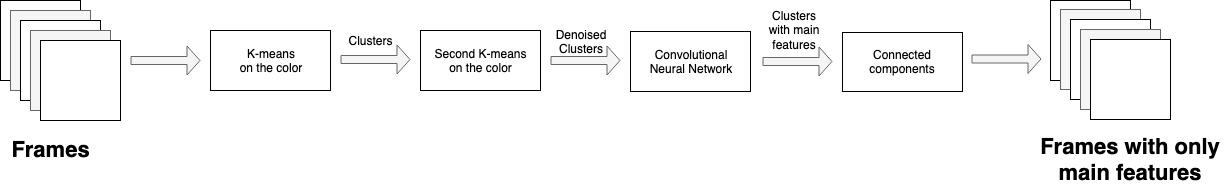
\includegraphics[width=0.95\linewidth]{img/smallflow}
	\caption{Workflow: extraction of the main components from the original frames}
	\label{fig:small}
\end{figure}
The first task to be completed is the application of the k-means clustering algorithm to the video, previously subdivided in frames. The goal is to be able to identify the main features among other secondary objects and obtain isolated clusters for each of them.
\newpage
\noindent
The next step consists in being able to distinguish between the clusters that contain the main items of the video and those that enclose  noisy components. In order to do that, we are going to use a convolutional neural network that is going to label all the generated clusters, identifying the ones that will be processed in the later stages. \\
 Each cluster classified as main component of the frame is then exposed to an algorithm that identifies all the connected components. The goal we want to reach is the partition of the cluster in its individual items.  \\
 The final step consists in reducing the overall run time of the routine, a task that is accomplished by executing the whole process in parallel for a suitable number of frames, depending on the number of processors available in the machine.
 The characteristics and the mathematical details behind the \textit{k}-means algorithm, convolutional neural network, connected components and multiprocessing are contained in section 2, while the results obtained by means of the application of previously listed methods are discussed in section 3.  \\
 
 
\section{Algorithms and Mathematical Background}
In order to apply the algorithms and adapt them to a specific problem it is fundamental to fully understand all the theoretical and mathematical concept characterizing their process. For this reason, before proceeding with the discussion and visualisation of the Video Segmentation Framework results, in this section it is presented the theoretical background of the methods used.

\subsection{\textit{k}-means clustering algorithm} 
In image segmentation, \textit{k}-means is one of the most popular clustering algorithms. It is intuitive, easy to implement and converges monotonically. In spite of this, \textit{k}-means presents also some drawbacks such as the fact that the number of clusters has to be known a priori and different initial seed can give rise to different outputs, because of the randomness of the initial component \cite{10}. \\
The algorithm uses an iterative approach, as represented in Figure \ref{fig:1} and formalized in Algorithm \ref{alg:1}. Starting from an initial set of random centroids, at each iteration it generates the clusters by minimizing the distance between each point and the centroids, based on a given proximity measure. Convergence is achieved when points are no longer interchanged between the clusters.
\begin{figure}[h]
	\centering
	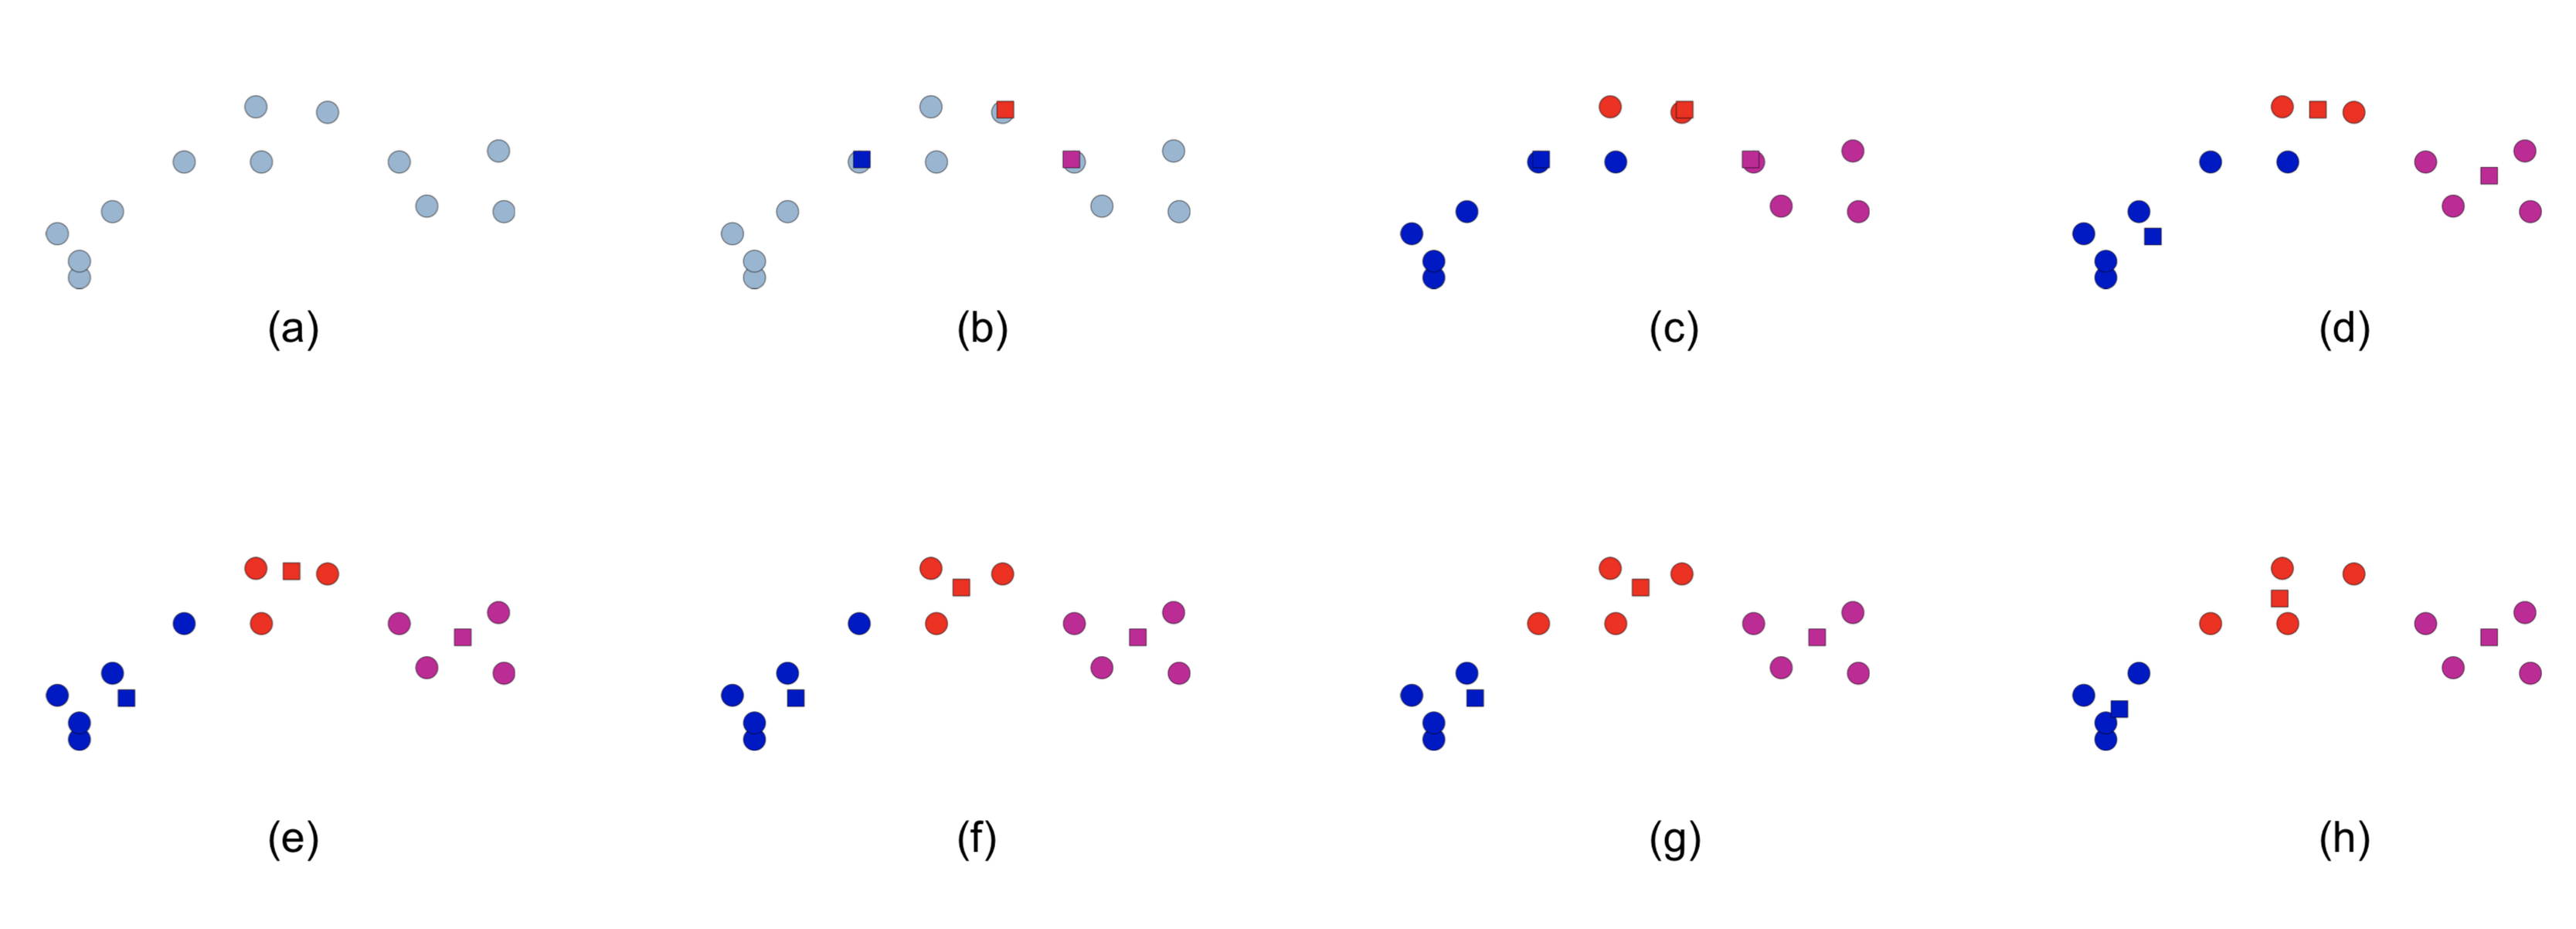
\includegraphics[scale=0.2]{./img/Kmeans_final}
	\caption{iterations of \textit{k}-means clustering algorithm applied to a group of datapoints (a) from initial random centroids (b) to final clusters (h). We can observe how the centre of mass is moving around, the points are assigned to clusters and the centroids are updated in (c)-(g)}
	\label{fig:1}
\end{figure}
\begin{algorithm}
	\caption{\textit{k}-means Clustering}\label{kmeans}
	\label{alg:1}
	\begin{algorithmic}[1]
		\Procedure{\textit{k}-means}{}
		\State Choose K random points as initial centroids 
		\While {not converged}
		\State Assemble K clusters by minimizing the distance between each point and centroids
		\State Compute new centroids
		\EndWhile
		\EndProcedure
	\end{algorithmic}
\end{algorithm} \\
\newpage
\noindent
The ultimate goal of the algorithm is to partition $N$ initial datapoints into \textit{k} clusters. Given the dataset $\left\lbrace x_1, x_2, \dots, x_N \right\rbrace$ we want to obtain a previously provided number \textit{k} of clusters denoted $\left\lbrace C_1, C_2, \dots, C_K \right\rbrace $. The objective function usually employed by \textit{k}-means is the Sum of Squared Errors, denoted as SSE. The aim  is to minimize SSE for a given set of centroids $c_k$ \cite{11}. \\
\textit{k}-means can be  formalized mathematically as follows: 
\begin{equation*}
\begin{split}
SSE(C) &= \sum_{k=1}^{K} \sum_{x_i \in C_k} \| x_i - c_k\|^2 \\ \\
c_k &= \frac{\sum\limits_{x_i \in C_k} x_i}{|C_k|}
\end{split}
\end{equation*}
Different proximity measures can be used when the \textit{k}-means algorithm is applied. The most popular one is the Euclidean distance metric. 
However in the particular case of this application the distance between the pixels is computed considering their colour in RGB format. This means that the data point $x_i$ will be represented by a three-dimensional array, which elements will correspond to the R, G, and B components of the colour. 

\subsection{Connected Components}
Connected components is a viable alternative to more common clustering algorithms, like \textit{k}-means. In order to understand how the algorithm works it is necessary to introduce some concepts of graph theory. \\
A graph $G=(V,E)$ is a set of elements $v \in V$ called vertices or nodes and a set of $e \in E$, the edges connecting the nodes. A path is a sequence of edges and vertices where each subsequent vertices are adjacent to each other and nor edges nor vertices are repeated \cite{12}. 
A connected component of an undirected graph (i.e. all edges are bi-directional)  is a subgraph where each two nodes are joint together by a path and at the same time  there is no connection with other nodes in the graph. 
Connected components is an algorithm that applies concepts of the graph theory in order to identify those sets of nodes that are considered similar based on a given heuristic. In particular, two nodes are considered part of the same connected component if there is a path between them, as represented in Figure \ref{fig:2}. \\
\begin{figure}[h]
	\centering
	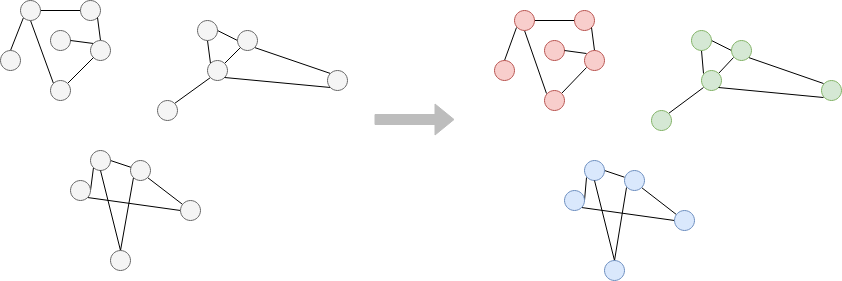
\includegraphics[width=0.6\linewidth]{img/conn_comp}
	\caption{An example of identification of 3 connected components in a graph with connected components algorithm}
	\label{fig:2}
\end{figure}
\newpage
\noindent
Identifying connected components could be a very useful tool if we want to isolate clusters in a set of items. 
The application of this algorithm on images will consider each pixel as one node of the graph. The metric used to evaluate the connection between two nodes is based on the colour of the pixels. A weighted alternative of the algorithm can also be considered. It recognizes two pixels in the same connected component if their distance in terms of colour is above a certain threshold.\\



\subsection{Convolutional Neural Network} 
A convolutional neural network is a deep learning algorithm that is usually applied in image processing \cite{13}.
Over the years, using convolutional neural networks have become the standard approach when it comes to image classification because of their speed and accuracy.
Like other neural network models, it consists of an input layer and an output layer, with several hidden layers in between.
The hidden layers of a CNN are usually convolutional layers, max-pooling layers, followed by some common fully connected layers.\\
The goal of the convolutional layer is to reduce the input size while maintaining the spatial relations of the pixels in the image. A convolutional layer takes as input a tensor, usually of shape batch-size $\times$ channels $\times$ height $\times$ width, and a kernel. The number of channels depends on the characteristics of the image: usually, taking into consideration the colour, there are three channels, that correspond to the three RGB values. 
On the other side, kernels define the output size of the layer and how the input image is processed. They can have different sizes and apply different functions to the pixels, depending on how they are defined.  \\
For example as shown in Figure \ref{fig:13}, considering a 3 $\times$ 3 kernel, a mask of the same dimension scans over the whole input image, pixel by pixel, computing the value in the centre with a weighted sum of all the pixels in the mask. The weights are defined by the selected kernel.

\begin{figure}[H]
	\centering
	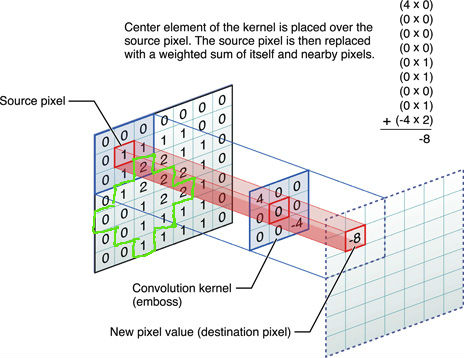
\includegraphics[width=0.5\linewidth]{img/kernel}
	\caption{A visual example of a convolutional layer with a 3$\times$3 kernel \cite{14}}
	\label{fig:13}
\end{figure}

\noindent
After the application of the convolutional layer, the goal of the pooling layer  is to further reduce the input size. However, it  is a lossy layer, meaning that it will not conserve all the information given by the input.
It usually divides the image in many 2$\times$2 groups of pixels and substitutes each of them with a single pixel, the one with the maximum  value. This halves the size of the image, as can be seen in \ref{fig:12}.
\begin{figure}[H]
	\centering
	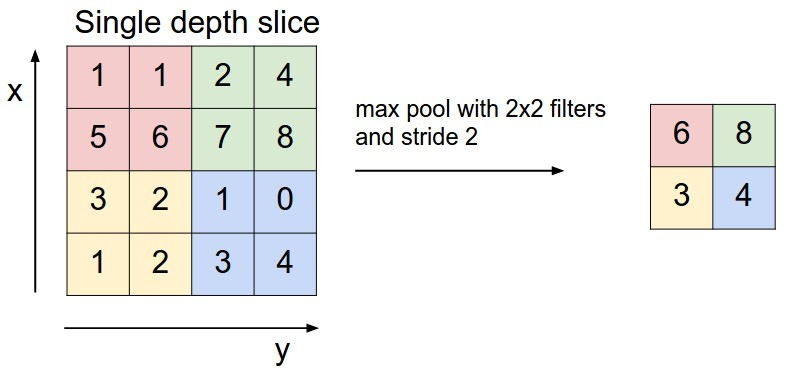
\includegraphics[width=0.4\textwidth]{img/maxpool}
	\caption{A visual representation of a max-pooling layer}
	\label{fig:12}
\end{figure}
\newpage
\noindent
The final step that leads to the classification is performed by a certain number of fully connected layers. As the name suggests, they are layers where each neuron is connected to all the neurons of the previous and the next layer. Each neuron carries a weight that is multiplied by the input, which is determined by the sum of all the incoming nodes. It results in an affine transformation of the input $X$ that can be mathematically formalized as
$$Y=X*W+b$$
where $Y$ is the output, $W$ is the matrix containing the neuron weights and $b$ is a constant value used to shift the result of the computation, called bias. 
%\begin{figure}[h]
%	\centering
%	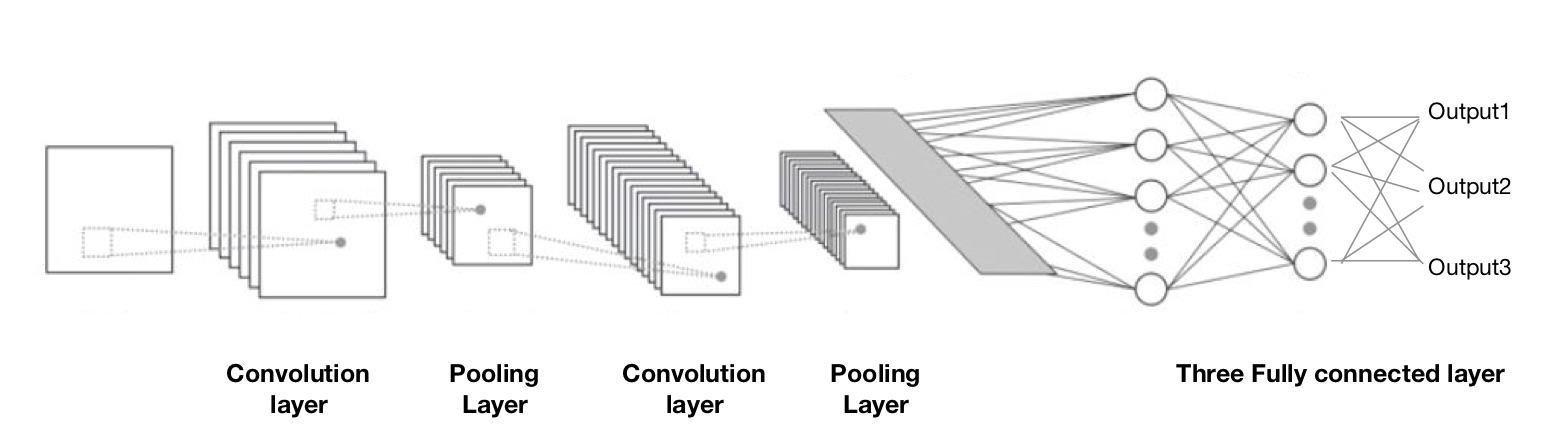
\includegraphics[width=0.98\linewidth]{img/cnn_gen}
%	\caption{}
%	\label{fig:cnngen}
%\end{figure}



\subsection{Multiprocessor parallelization}
Multiprocessors refers to the use of two or more CPUs (central processing units) contained in a single computer system that supports the execution of threads collaborating on a single task. The coordination and the usage of the single processors is controlled by the same operating system and all the processors share the same main memory by means of a shared address space.  \\
The usage of multiple processors instead of one presents several advantages. One of the most important ones is the increasing of the  throughput, which means that more work can be executed and completed in a unit time. However, an important drawback could be the cost of the communication among different processors. For this reason the parallelization of a program with multiprocessing is particularly convenient if the tasks are independent of each other.

\begin{figure}[h]
	\centering
	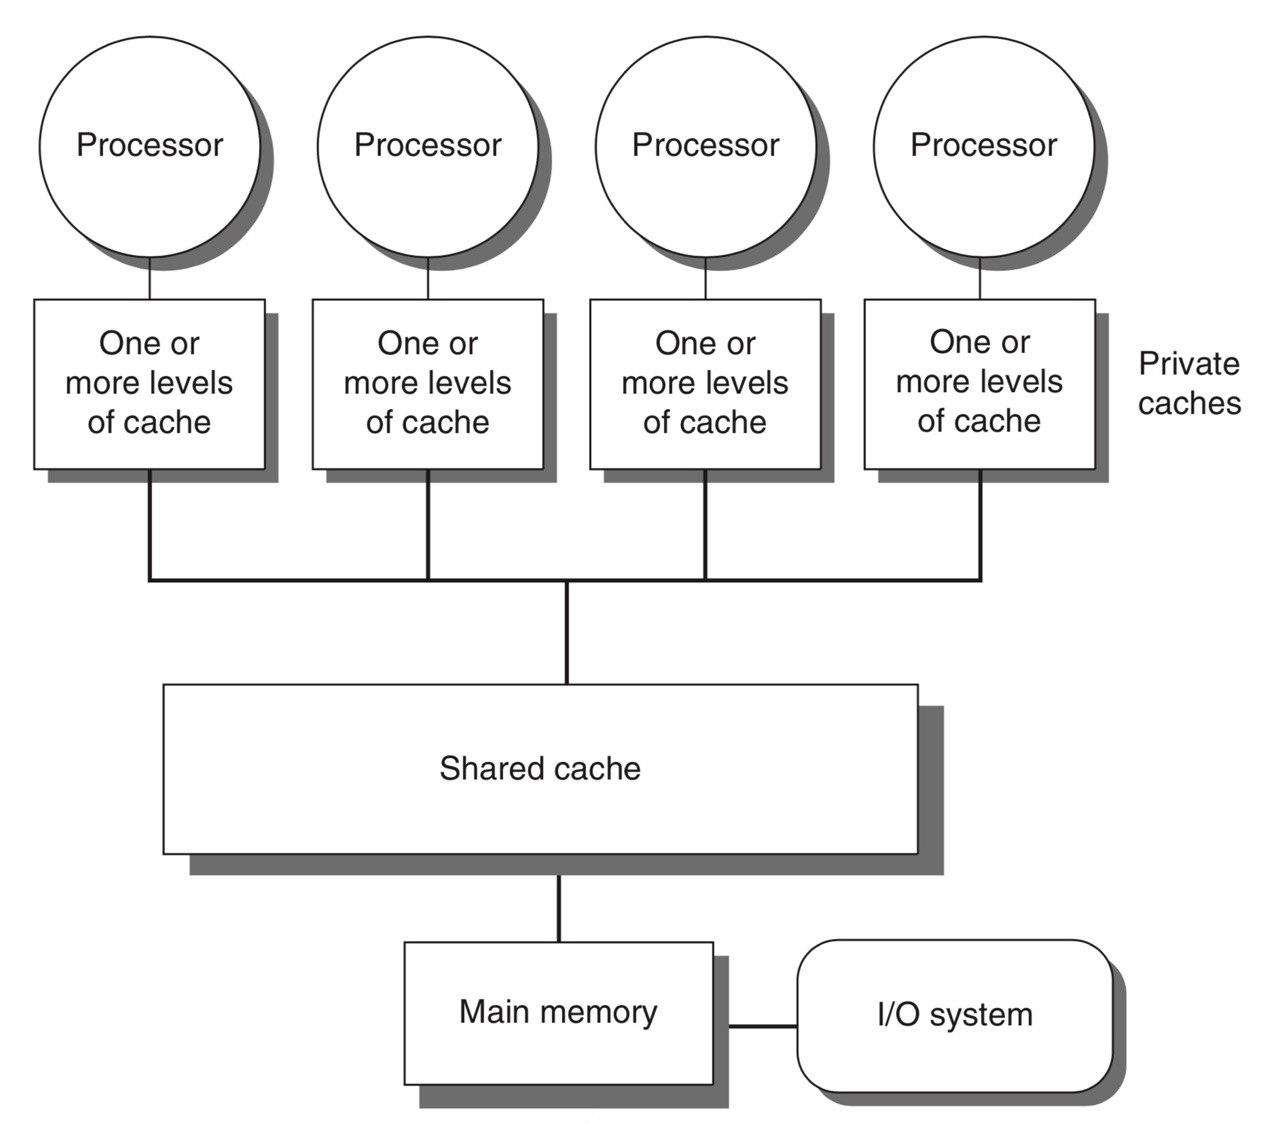
\includegraphics[width=0.35\linewidth]{img/multiprocessing}
	\caption{Structure of a centralized shared-memory multiprocessor \cite{15}}
	\label{fig:3}
\end{figure}



\section{Results \& Discussion}
This section presents, step by step, the results of the High Performance Video Segmentation Framework, obtained by applying the methods previously discussed to a specific case. The way the algorithms are adapted and manipulated in order to fit the test case is also examined. 

\subsection{Test Case}
The specific video we are considering represents a clip of a billiard game with a duration of about 2 minutes, filmed with a static camera. The video subdivided in frames generates 3582 images, some examples of which are shown in Figure \ref{fig:4}. Each frame has dimension of $1280 \times 720$,  for a total of 921'600 pixels. \\
\begin{figure}[h]
	\centering
	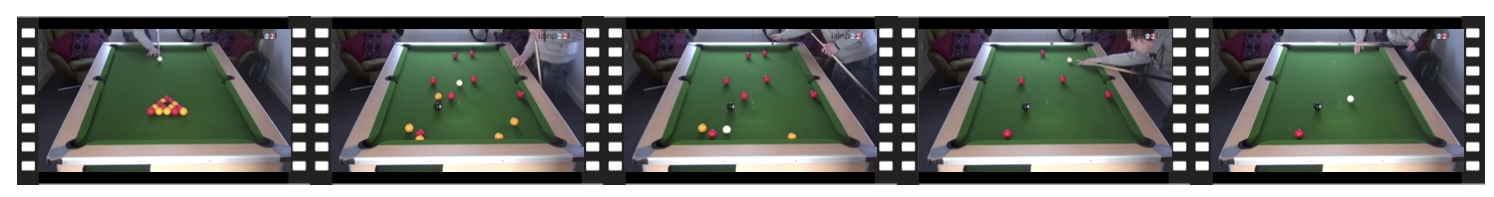
\includegraphics[width=0.98\linewidth]{img/video_frames}
	\caption{Examples of frames extracted from 5 different moments of the footage}
	\label{fig:4}
\end{figure}

\noindent
In the video there are two teams represented by red and yellow balls; the aim of the application is to separate and identify the members of each team. The final goal is to reassemble the video with only its main features, represented by the single balls and display a counter to keep track of each team's members left on the table. 

\subsection{Video Feature Extraction}
We hereby suggest an effective approach to perform video feature extraction. All the methods described are applied to all the single frames of the clip, but for the sake of brevity only one example will be presented.  \\
Once the frames are extracted from the video by means of the OpenCV library for Python, the \textit{k}-means algorithm is applied to them for the first time in order to separate the main features from those of less interest. However, before applying the clustering algorithm to the frames it is convenient to get rid of the possible influence of the secondary objects. For this purpose the background will be set to black on each frame before proceeding with the analysis. \\
The clustering algorithm is performed using the function \texttt{kmeans} from the OpenCV library. The main parameters given in input are the vectorized image, the number of clusters, the termination criteria  and the flag specifying how the initial centroids are chosen. The image is transformed into a number of pixels$\times 3$ array containing the RGB values; the number of clusters is set to 5 because the initial idea was to identify red balls, yellow balls, white ball, table and background. 
In Figure \ref{fig:5} it can be observed how the algorithm divides the image in its main components based on the colour; the result is not exactly as expected. 

\begin{figure}[h]
	\centering
	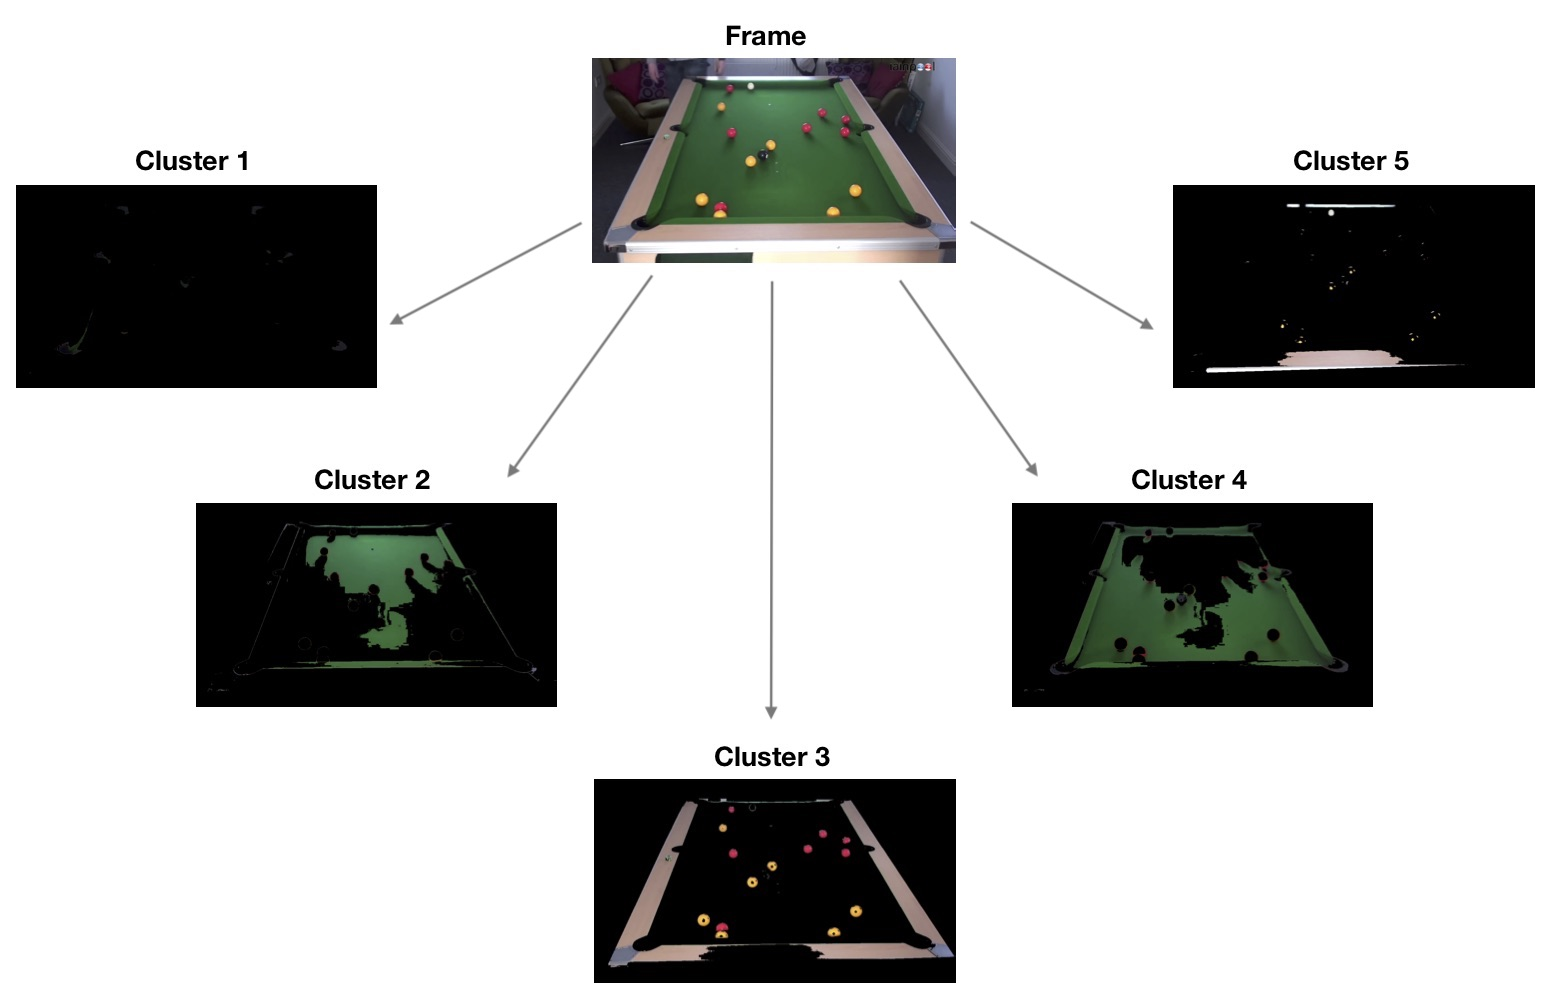
\includegraphics[width=0.7\linewidth]{./img/cluster1}
	\caption{The clusters resulting from the first application of \textit{k}-means algorithm}
	\label{fig:5}
\end{figure}
\noindent
As previously stated, the result wanted from the application of the \textit{k}-means algorithm was the separation of the members of each team in two different clusters. However, it is easy to notice that this task has not been accomplished in the previous step. In spite of this, we have obtained a cluster that contains the member of the two teams, i.e. cluster number 3, and a second application of the \textit{k}-means algorithm can give rise to the division of the teams in two different clusters. \\
Since there is no way to know in which order the clusters will be generated and therefore it is impossible to identify the cluster that contains the teams, the \textit{k}-means clustering will be applied for the second time to all the resulting frames from the previous step. As before, the algorithm generates 5 clusters from each input, identifying the two teams and removing the noise, as represented in  Figure \ref{fig:6}. \\
\begin{figure}[h]
	\centering
	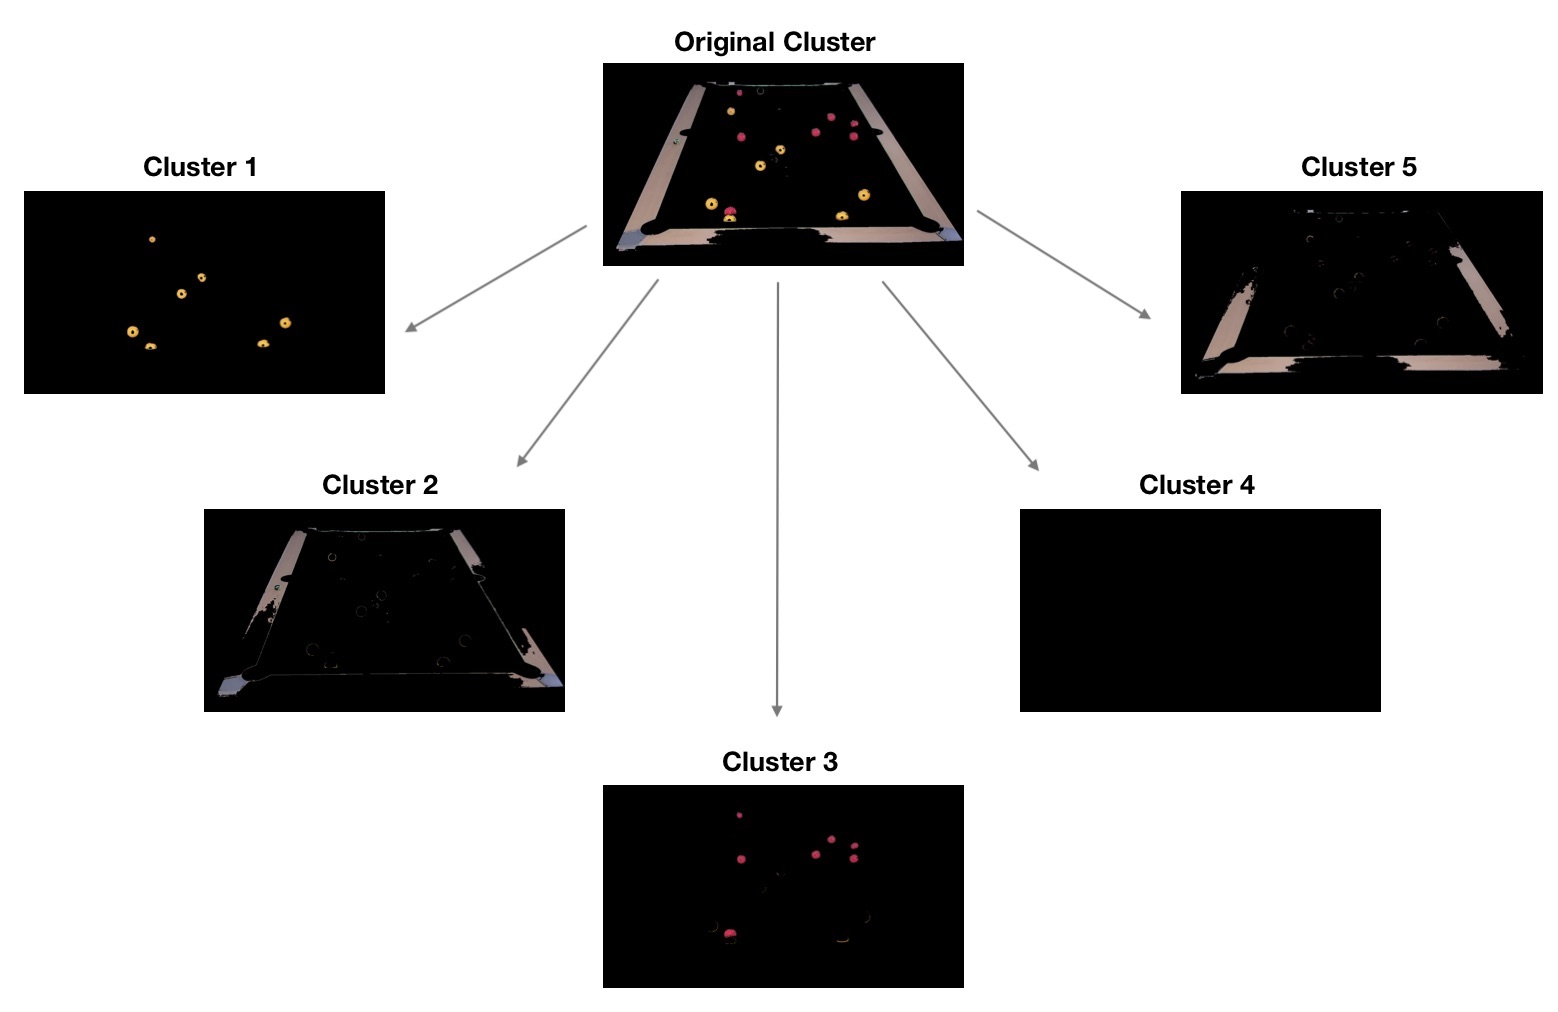
\includegraphics[width=0.7\linewidth]{./img/clusters2}
	\caption{The clusters resulting from the second application of \textit{k}-means algorithm to Cluster 3 from Figure \ref{fig:5}}
	\label{fig:6}
\end{figure}

\noindent
From the double application of \textit{k}-means algorithm we obtain 25 clusters; the next goal will be identifying which of them contain the main features, i.e. the two teams. \\
In order to achieve this result we have used a Convolutional Neural Network, trained to classify a cluster as yellow team, red team or noise. The training is performed based on a set of 500 frames classified manually. The precision achieved is over 99\%.
\newpage
\noindent
Once the two teams have been identified and labelled by the convolutional neural network, the next goal is to identify each member of the two teams, separating them, as can be observed in Figure \ref{fig:7}, by applying the connected components algorithm. This will allow to keep track of the trajectory of every single member and identify the number of balls present on the billiard table.
\begin{figure}[h]
	\centering
	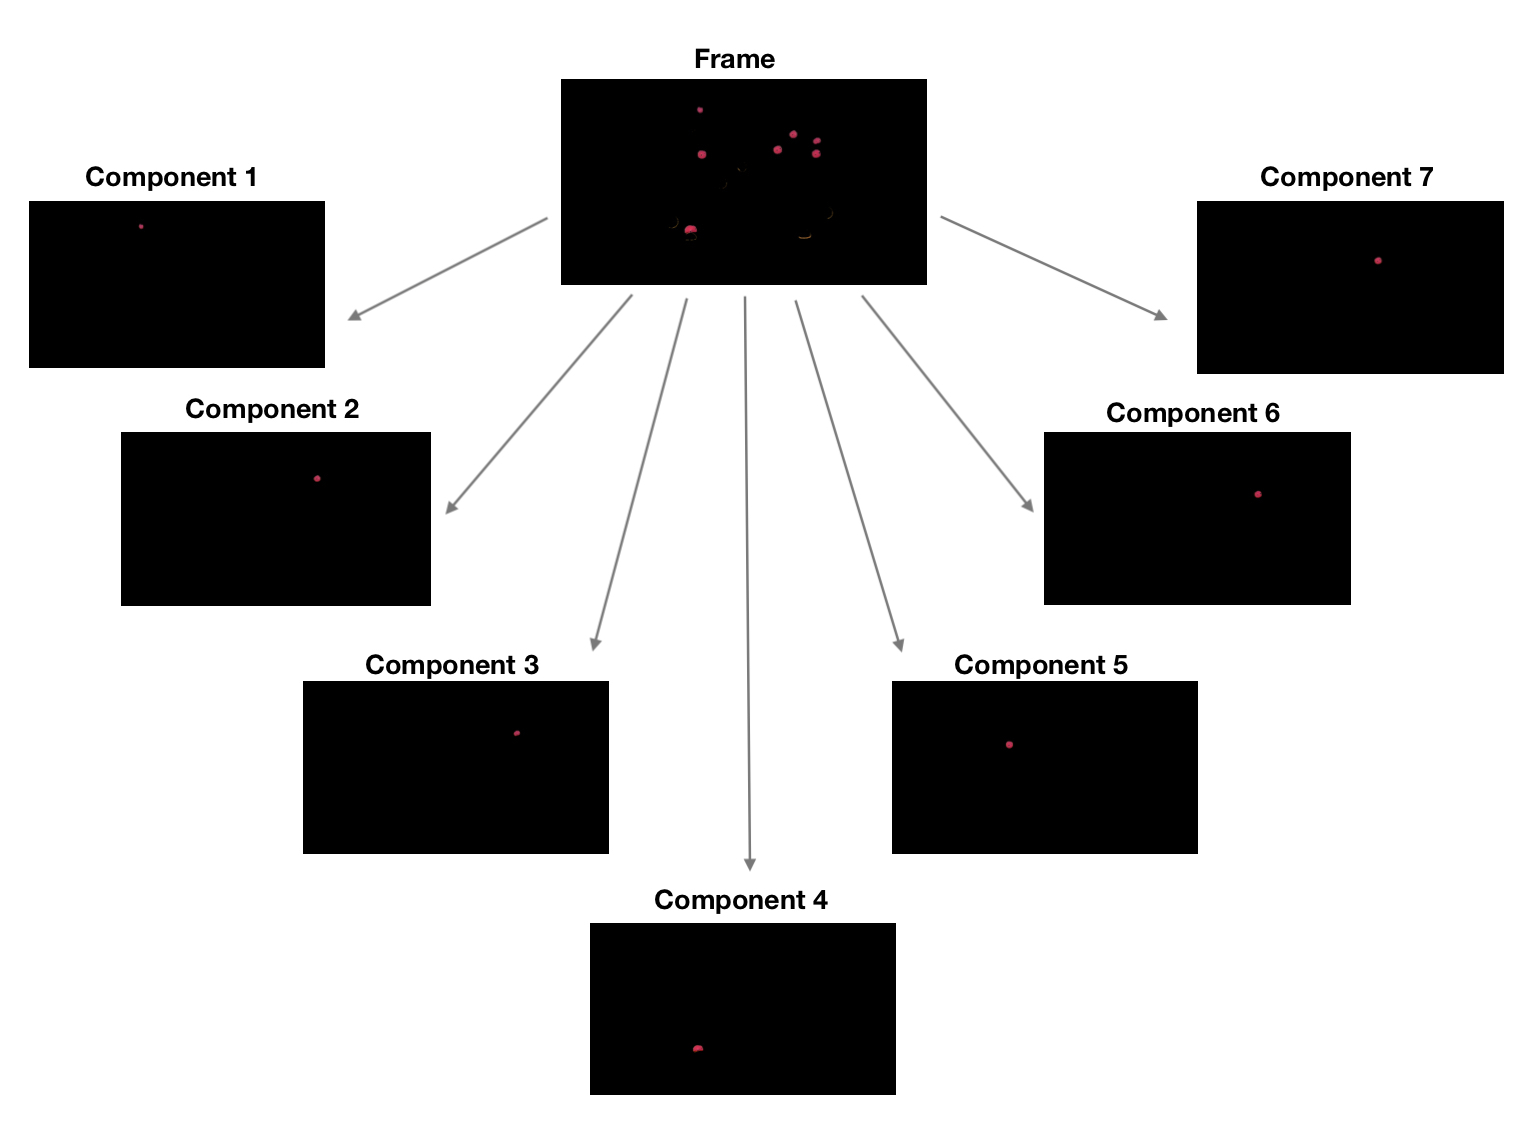
\includegraphics[width=0.7\linewidth]{./img/cc}
	\caption{The clusters resulting from the application of the connected components algorithm applied to the Cluster 3 of Figure \ref{fig:6}}
	\label{fig:7}
\end{figure}

\noindent
The connected component clustering is performed by the SciPy library that employs a Gaussian filter and a function that labels features in an array based on a threshold that in this particular case was set to 50. \\
Once the connected components are identified the frame is reassembled, as shown in Figure \ref{fig:8}. 
\begin{figure}[h]
	\centering
	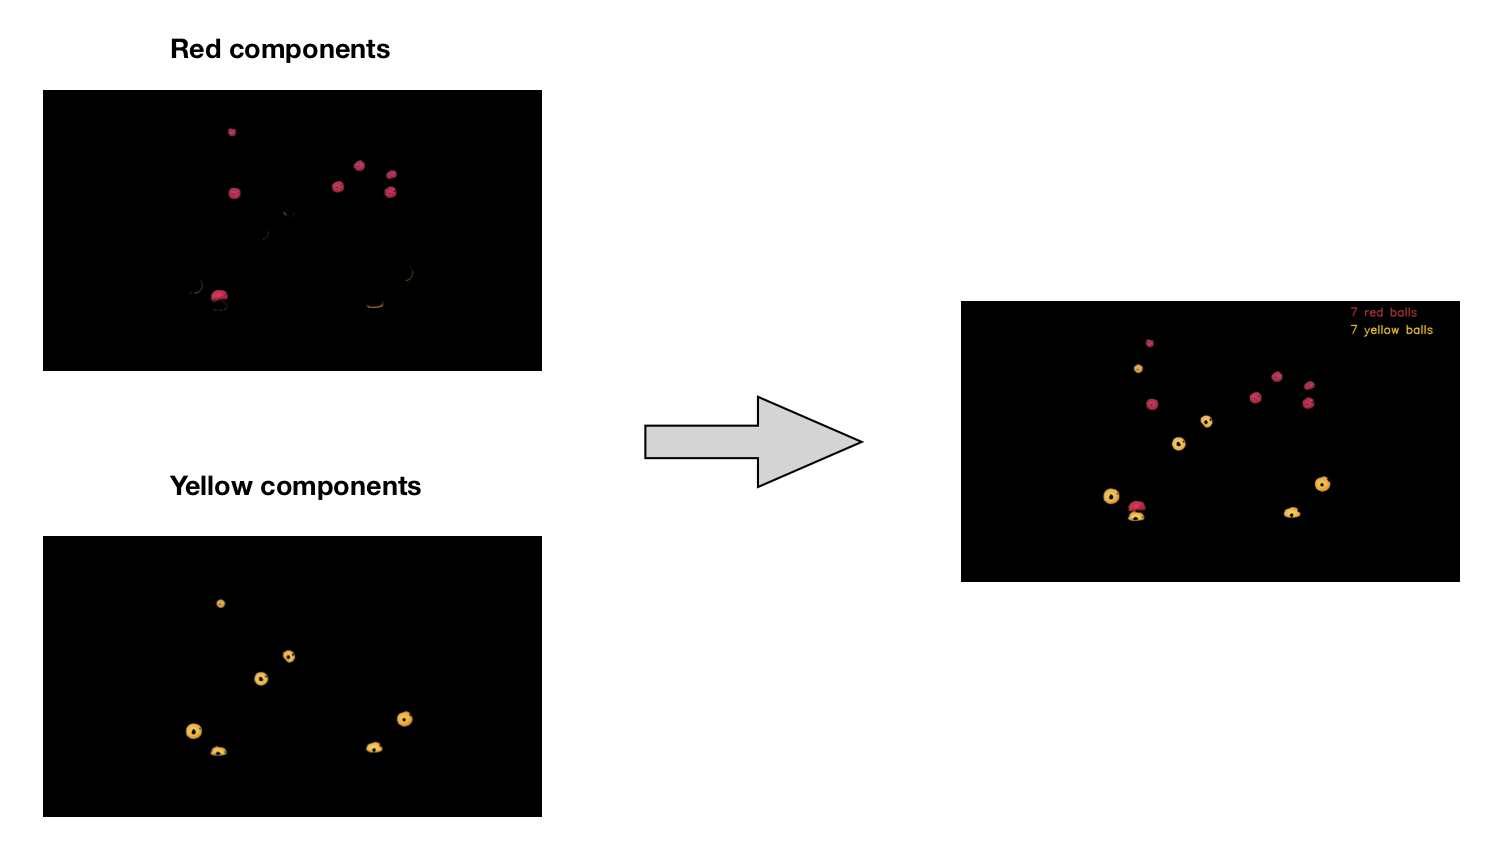
\includegraphics[width=0.7\linewidth]{./img/to_frame}
	\caption{The reassembled frame with counter}
	\label{fig:8}
\end{figure}

\noindent
After this procedure is applied to each frame, the final video is reassembled with only the members of the two teams, displaying the balls counter, as visualized in Figure \ref{fig:10}. 
\begin{figure}[h]
	\centering
	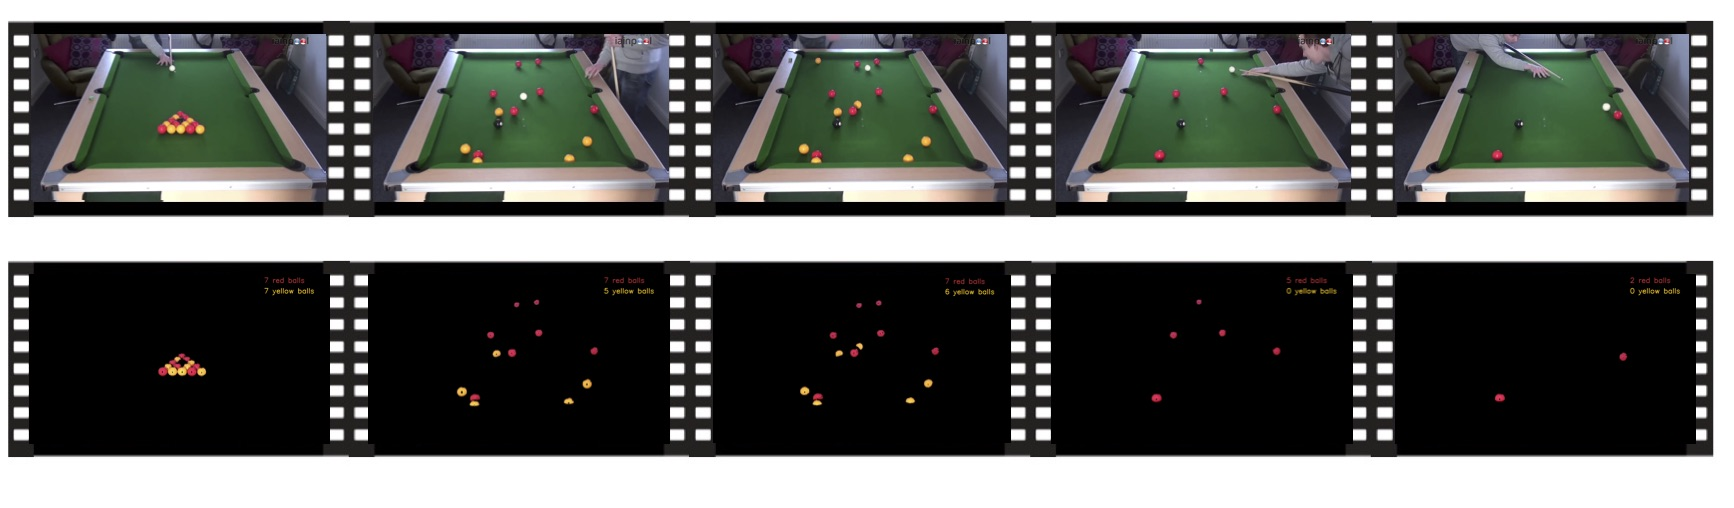
\includegraphics[width=1\linewidth]{./img/frames}
	\caption{The reassembled frame with counter}
	\label{fig:10}
\end{figure}


\newpage
\subsection{Parallelization \& Scalability}
All the processes explained until now, applied to a single frame take about 94 seconds to execute on a MacBook Pro with a 2.2 GHz Intel Core i7 processor and a memory of 16 GB 2400 MHz DDR4. So, to run the feature extraction techniques on all the frames on this machine would require 336'708 seconds, i.e. almost 94 hours. For this reason, the framework has been parallelized and can be run on multiple processors, due to the independence of the frames. For these simulations, the ICS cluster that is composed of 42 nodes, is used. Our application is run on regular nodes, with 2 CPUs Intel Xeon E5-2650 v3 @ 2.30GHz, 20 cores and a RAM of 64GB DDR4 @ 2133MHz each. \\
In order to show the scalability of the Video Segmentation Framework, it is run on 1, 2,4,8 and 16 nodes. It can be observed in Figure \ref{fig:9} that by increasing the number of nodes the execution time reduces significantly and almost ideally, i.e. doubling the number of cores the execution time halves. Because of the limited resources, the point of saturation, i.e. when the program has no more improvement in execution time increasing the number of nodes, could not be shown.

\begin{figure}[h]
	\centering
	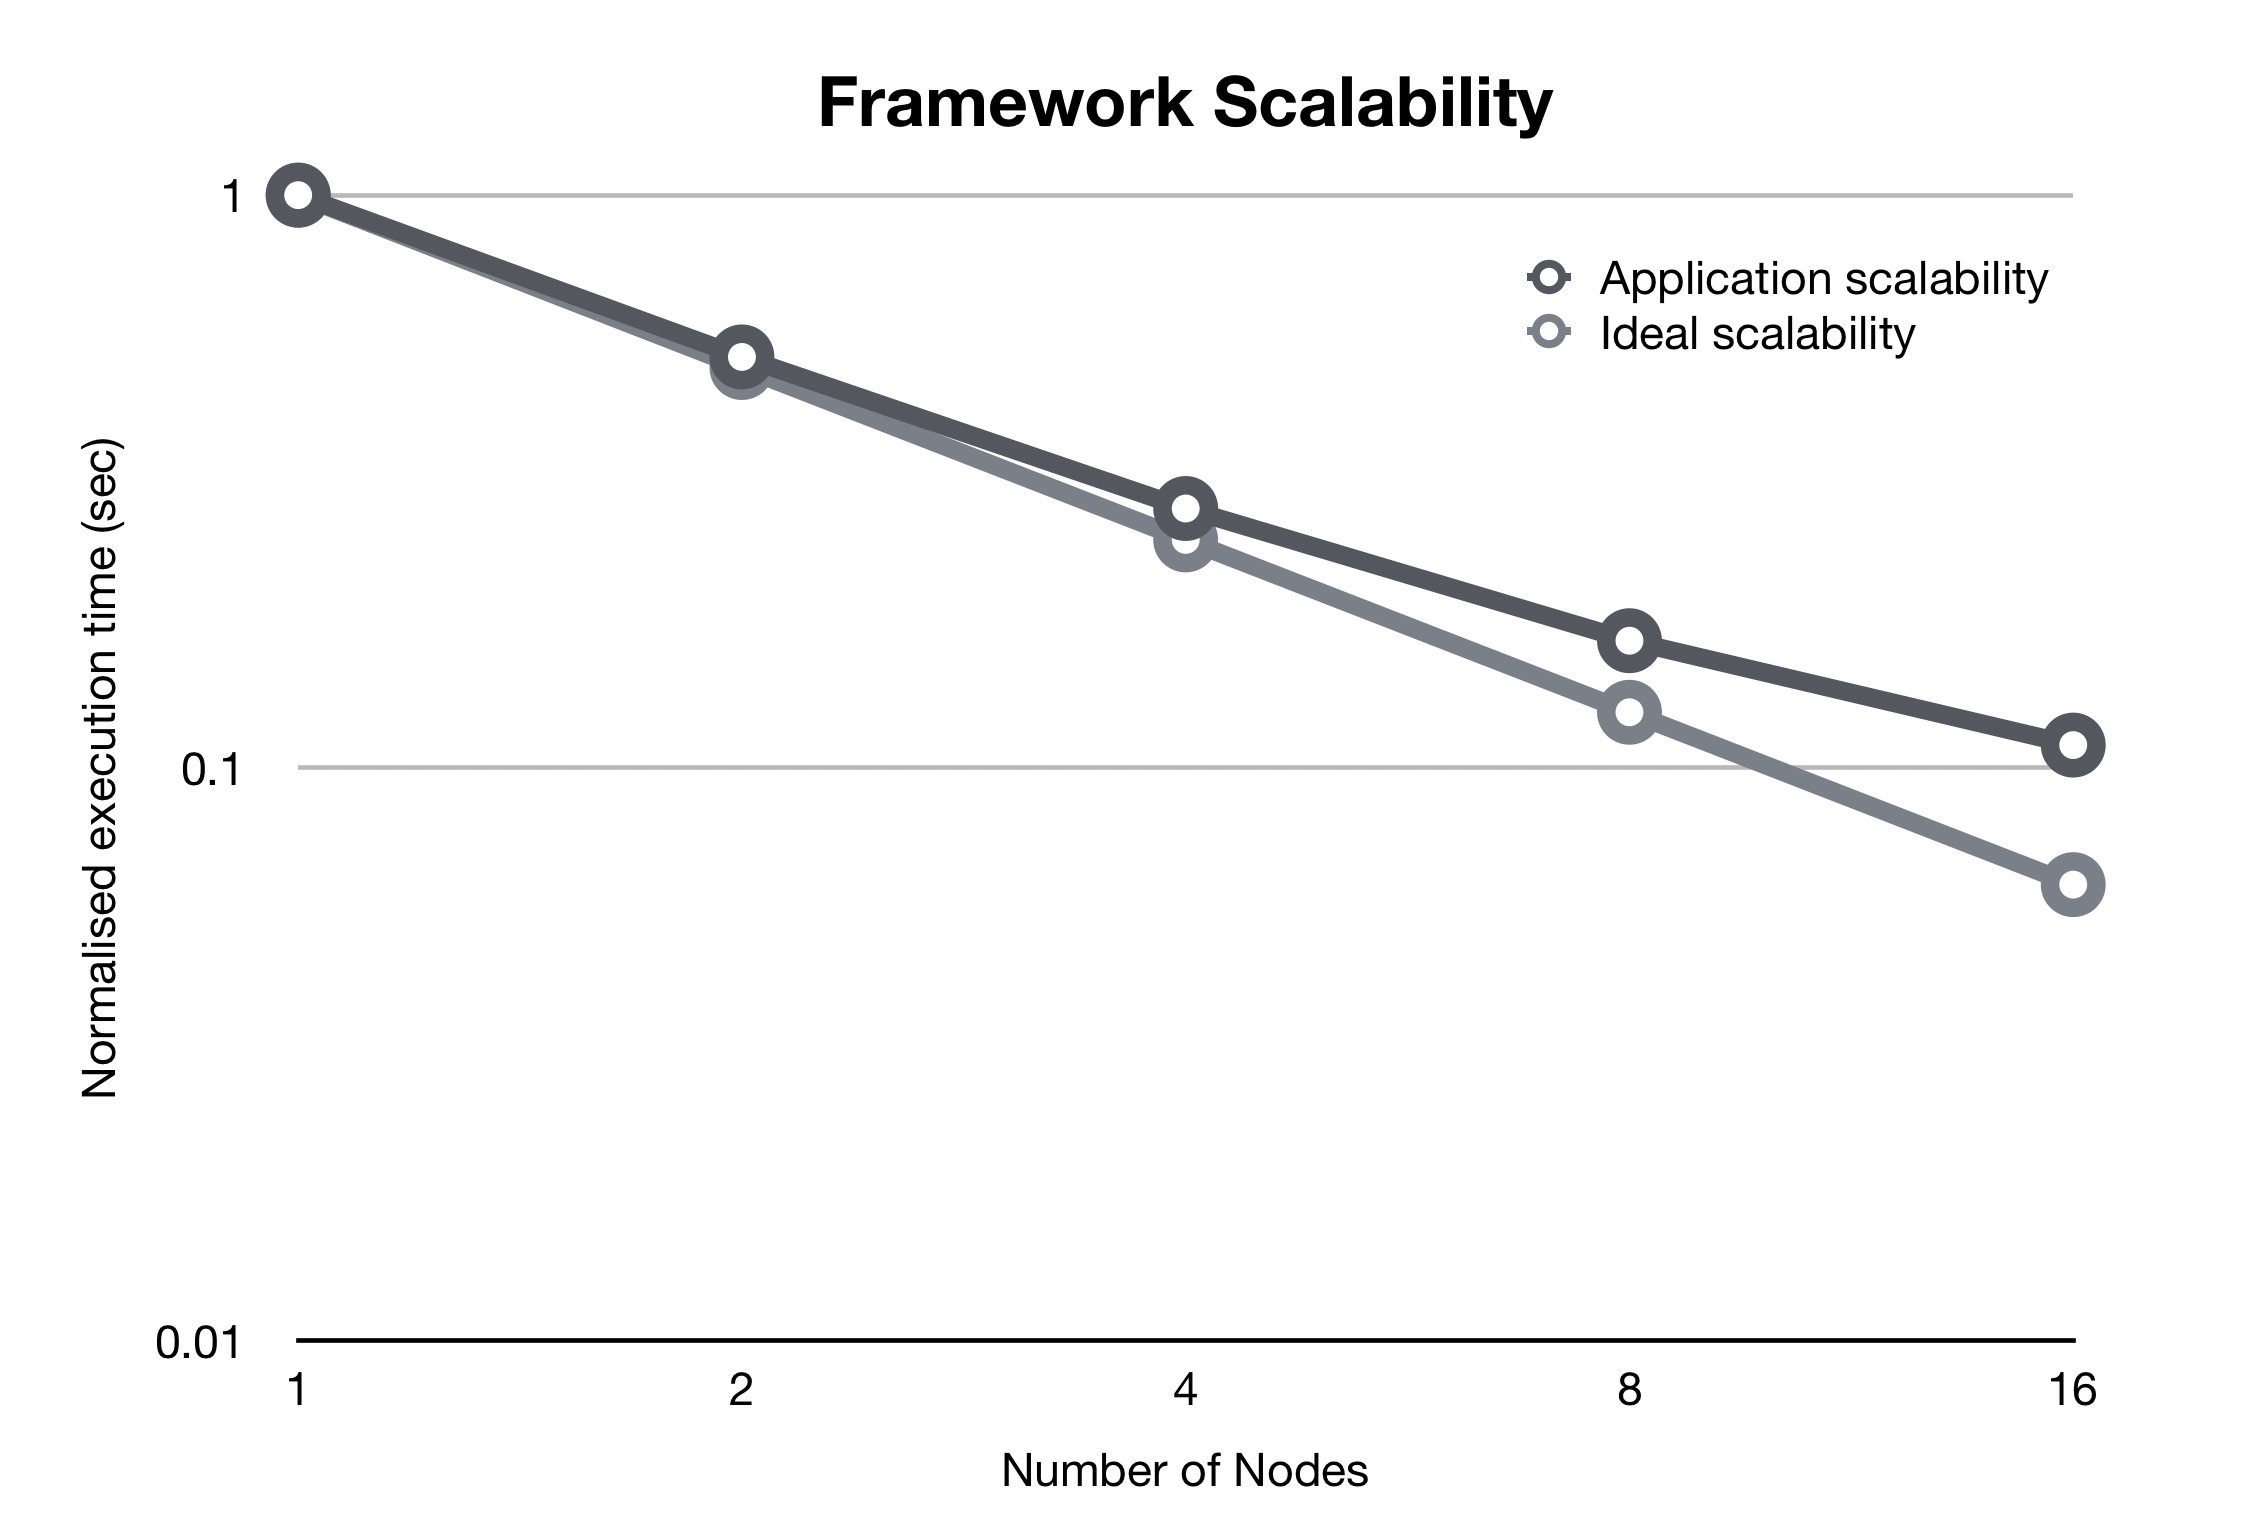
\includegraphics[width=0.8\linewidth]{img/scalability}
	\caption{Framework Scalability: execution time versus number of nodes}
	\label{fig:9}
\end{figure}

\newpage
\section{Conclusion \& Future work }
The presented work is an efficient approach to the video segmentation problem. It is based on the employment of fast and inexpensive techniques that successfully identify the critical components of a video. \\
The main steps characterizing the High Performance Video Segmentation Framework are 
\begin{itemize}
	\item[(i)] the double application of the \textit{k}-means algorithm to the frames of a video, 
	\item[(ii)] the classification of the resulting clusters in three groups (i.e. yellow team, red team and noise), 
	\item[(iii)] the application of the connected components clustering algorithm to identify the single members of each team
	\item[(iv)] and finally, the reassembly of the video with only its main features (the two teams). \\
\end{itemize}
Experimental results show that the method proposed leads to an efficient identification and feature extraction of the main objects in a video. The application is computationally inexpensive but could require a long execution time in the case of long videos that generate thousands of frames. This issue can be easily overcome by the fact that when the program is executed on multiple processors it has an almost ideal scalability that reduces significantly the runtime. \\
Future work could develop in different directions. A first option for a further evolution could be the employment of more powerful clustering algorithm such as Spectral clustering, in order to improve the quality of the clusters obtained. In another possible development, the framework can be manipulated and adapted in order to fit different test cases; possible applications could be various types of sports and the identification of potential obstructive objects in autonomous vehicles.

\bibliographystyle{unsrt}  
%\bibliography{references}  %%% Remove comment to use the external .bib file (using bibtex).
%%% and comment out the ``thebibliography'' section.


%%% Comment out this section when you \bibliography{references} is enabled.
\newpage
\begin{thebibliography}{1}
	
	
	\bibitem {1}
	B.V. Patel and B.B. Meshram,
	\textit{Content Based Retrieval Systems},
	International Journal of UbiComp (IJU), Vol.3, No.2, 
	April 2012
	
	\bibitem {2} 
	H. Cho, Y. Seo, B. V. K. V. Kumar and R. R. Rajkumar, 
	\textit{A multi-sensor fusion system for moving object detection and tracking in urban driving environments}, 
	IEEE International Conference on Robotics and Automation (ICRA), 
	2014
	
	\bibitem {3} 
	Ed-Edily Mohd,  Azhari,Muhd. Mudzakkir Mohd. Hatta, Zaw Zaw Htike,  Shoon Lei Win, 
	\textit{Tumor detection in medical imaging: a survey }, 
	International Journal of Advanced Information Technology (IJAIT) Vol. 4, No. 1, 
	February 2014
	
	\bibitem{4}
		Elnemr Heba Zayed, Nourhan Fakhreldein Mahmoud, 
		\textit{Feature Extraction Techniques: Fundamental Concepts and Survey},
		Handbook of Research on Emerging Perspectives in Intelligent Pattern Recognition, Analysis, and Image Processing, Chapter: 13,
		January 2016
		
	\bibitem{5}
		Dong ping  Tian, 
		\textit{A Review on Image Feature Extraction and Representation Techniques},
		International Journal of Multimedia and Ubiquitous Engineering,
		July 2013
		
	\bibitem{6}
		Mark Nixon and Alberto Aguado, 
		\textit{Feature Extraction and Image Processing for Computer Vision} Third edition,
		2012
		
	\bibitem{7}
		Nameirakpam Dhanachandra, Khumanthem Manglem, Yambem Jina Chanu,  
		\textit{Image Segmentation Using K -means Clustering Algorithm and Subtractive Clustering Algorithm} 
		Procedia Computer Science, Volume 54,
		2015
		
	\bibitem{8}
		Zhensong Chen, Zhiquan Qi, Fan Meng, Limeng Cui, Yong Shi,
		\textit{Image Segmentation via Improving Clustering Algorithms with Density and Distance} 
		Procedia Computer Science,
Volume 55
		2015,
		
	\bibitem{9}
		E.J Pauwels, G Frederix,
		\textit{Finding Salient Regions in Images: Nonparametric Clustering for Image Segmentation and Grouping} 
		Computer Vision and Image Understanding, Volume 75,
		1999
	
	\bibitem{10}
		A. Oliver, X. Munoz, J. Batlle, L. Pacheco and J. Freixenet
		\textit{Improving Clustering Algorithms for Image Segmentation using Contour and Region Information},
		2006 IEEE International Conference on Automation, Quality and Testing, Robotics,
		2006
	\bibitem{11}
		Charu C. Aggarwal  and Chandan K. Reddy
		\textit{Data Clustering, Algorithms and Applications},Chapter 4,
		2014
	\bibitem{12}
		Robin J. Wilson
		\textit{Introduction to graph theory}, Fifth edition
		2010
	\bibitem{13}
		John L. Hennessy, David A. Patterson,
		\textit{Guide to Convolutional Neural Networks. A Practical Application to Traffic-Sign Detection and Classification}, First edition,
		2017
	\bibitem{14}
		Loris Foresti, Pascal Horton
		\textit{Filtres et convolution}, UNIL,
		2015
	\bibitem{15}
		Hamed Habibi Aghdam ans Elnaz Jahani Heravi
		\textit{Computer architecture: a quantitative approach}, Fifth edition,
		2012
\end{thebibliography}


%%%%%%%%%%%%%%%%%%%%%%%%%%%%%%%%%%%%%%%%%%%%%%%%%%%%%%%%%%%%%%%%%%%%

\end{document}
